
\documentclass[border=10pt, 12pt]{standalone}
\usepackage[svgnames]{xcolor}
\usepackage{amsmath}
\usepackage{pgfplots}
\pgfplotsset{compat=newest}
\usepackage[sfdefault]{FiraSans}
\usepackage{FiraMono}
\renewcommand*\familydefault{\sfdefault}
\begin{document}
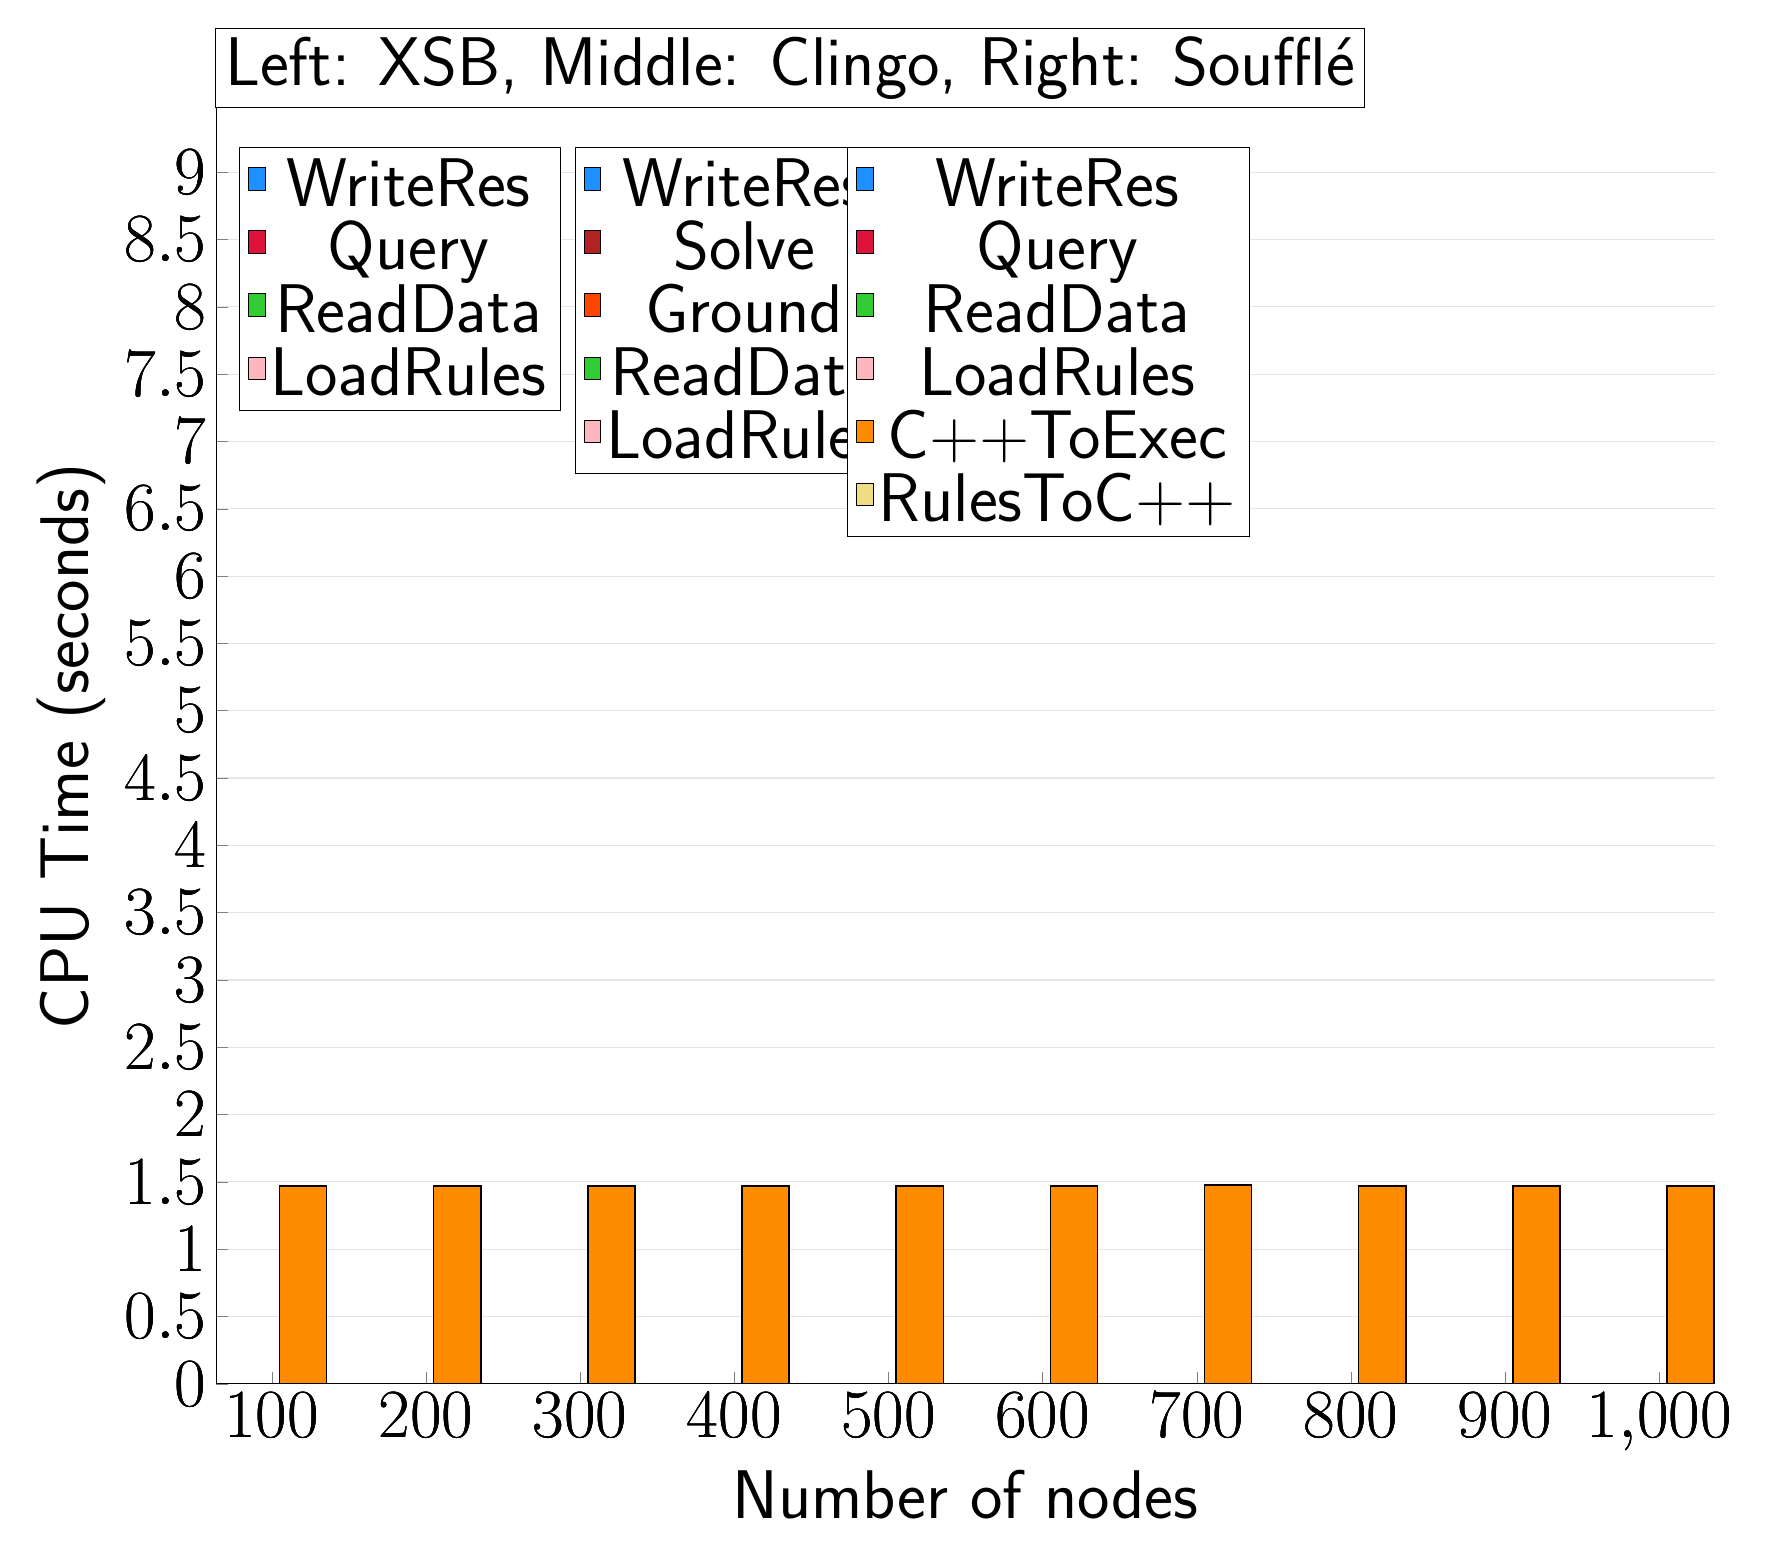
\begin{tikzpicture}
                        \begin{axis}[bar shift=-24.3pt, 
   ybar stacked,
   width=1.7\textwidth,
   bar width=0.6cm,
   ymajorgrids, tick align=inside,
   major grid style={draw=gray!20},
   xtick=data,
   ymin=0, ymax=9.474,
   axis x line*=bottom,
   axis y line*=left,
   enlarge x limits=0.04,
   legend style={
       at={(0.23, 0.97)},
       anchor=north east,
       legend columns=1,
       font=\Huge,
   },
   ylabel={CPU Time (seconds)},
   xlabel={Number of nodes},
   label style={font=\Huge},
   tick label style={font=\Huge},
]
\addlegendimage{fill=DodgerBlue, draw=black, line width=0.2pt}
\addlegendentry{WriteRes}
\addlegendimage{fill=Crimson, draw=black, line width=0.2pt}
\addlegendentry{Query}
\addlegendimage{fill=LimeGreen, draw=black, line width=0.2pt}
\addlegendentry{ReadData}
\addlegendimage{fill=LightPink, draw=black, line width=0.2pt}
\addlegendentry{LoadRules}
\addplot +[fill=LightPink, draw=black, line width=0.55pt] coordinates {
(100, 0.0005502)
(200, 0.0005495999999999994)
(300, 0.0005480000000000002)
(400, 0.0005483999999999996)
(500, 0.0005520000000000006)
(600, 0.0005464)
(700, 0.0005485999999999998)
(800, 0.0005479999999999999)
(900, 0.0005496000000000001)
(1000, 0.0005504000000000002)
};
\addplot +[fill=LimeGreen, draw=black, line width=0.55pt] coordinates {
(100, 0.0001944000000000002)
(200, 0.00026720000000000015)
(300, 0.0003433999999999996)
(400, 0.00041699999999999984)
(500, 0.00048719999999999986)
(600, 0.0005637999999999996)
(700, 0.000639)
(800, 0.0007104000000000002)
(900, 0.0007878000000000003)
(1000, 0.0008636)
};
\addplot +[fill=Crimson, draw=black, line width=0.55pt] coordinates {
(100, 1.6599999999999638e-05)
(200, 2.440000000000046e-05)
(300, 3.480000000000007e-05)
(400, 4.580000000000036e-05)
(500, 5.48e-05)
(600, 6.520000000000031e-05)
(700, 7.49999999999997e-05)
(800, 8.559999999999956e-05)
(900, 9.319999999999988e-05)
(1000, 0.0001015999999999999)
};
\addplot +[fill=DodgerBlue, draw=black, line width=0.55pt] coordinates {
(100, 0.00014500000000000038)
(200, 0.00022839999999999934)
(300, 0.00031099999999999954)
(400, 0.0003939999999999998)
(500, 0.0004772000000000004)
(600, 0.0005645999999999996)
(700, 0.0006455999999999999)
(800, 0.0007306000000000002)
(900, 0.0008209999999999999)
(1000, 0.0008987999999999996)
};
\end{axis}

\begin{axis}[bar shift=-6.5pt, 
   ybar stacked,
   width=1.7\textwidth,
   bar width=0.6cm,
   ymajorgrids, tick align=inside,
   major grid style={draw=none},
   xtick=data,
   ymin=0, ymax=9.474,
   axis x line*=none,
   axis y line*=none,
   enlarge x limits=0.04,
   legend style={
       at={(0.454, 0.97)},
       anchor=north east,
       legend columns=1,
       font=\Huge,
   },
   label style={font=\Huge},
   tick label style={font=\Huge},
]
\addlegendimage{fill=DodgerBlue, draw=black, line width=0.2pt}
\addlegendentry{WriteRes}
\addlegendimage{fill=FireBrick, draw=black, line width=0.2pt}
\addlegendentry{Solve}
\addlegendimage{fill=OrangeRed, draw=black, line width=0.2pt}
\addlegendentry{Ground}
\addlegendimage{fill=LimeGreen, draw=black, line width=0.2pt}
\addlegendentry{ReadData}
\addlegendimage{fill=LightPink, draw=black, line width=0.2pt}
\addlegendentry{LoadRules}
\addplot +[fill=LightPink, draw=black, line width=0.55pt] coordinates {
(100, 0.0)
(200, 0.0)
(300, 0.0)
(400, 0.0)
(500, 0.0)
(600, 0.0)
(700, 0.0)
(800, 0.0)
(900, 0.0)
(1000, 0.0)
};
\addplot +[fill=LimeGreen, draw=black, line width=0.55pt] coordinates {
(100, 0.0)
(200, 0.0)
(300, 0.0)
(400, 0.0)
(500, 0.0)
(600, 0.0)
(700, 0.0)
(800, 0.0)
(900, 0.0)
(1000, 0.0)
};
\addplot +[fill=OrangeRed, draw=black, line width=0.55pt] coordinates {
(100, 0.0)
(200, 0.0)
(300, 0.0)
(400, 0.0)
(500, 0.0)
(600, 0.0)
(700, 0.0)
(800, 0.0)
(900, 0.0)
(1000, 0.0)
};
\addplot +[fill=FireBrick, draw=black, line width=0.55pt] coordinates {
(100, 0.0)
(200, 0.0)
(300, 0.0)
(400, 0.0)
(500, 0.0)
(600, 0.0)
(700, 0.0)
(800, 0.0)
(900, 0.0)
(1000, 0.0)
};
\addplot +[fill=DodgerBlue, draw=black, line width=0.55pt] coordinates {
(100, 0.0)
(200, 0.0)
(300, 0.0)
(400, 0.0)
(500, 0.0)
(600, 0.0)
(700, 0.0)
(800, 0.0020000000000000018)
(900, 0.0)
(1000, 0.0)
};
\end{axis}

\begin{axis}[bar shift=11.3pt, 
   ybar stacked,
   width=1.7\textwidth,
   bar width=0.6cm,
   ymajorgrids, tick align=inside,
   major grid style={draw=none},
   xtick=data,
   ymin=0, ymax=9.474,
   axis x line*=none,
   axis y line*=none,
   enlarge x limits=0.04,
   legend style={
       at={(0.69, 0.97)},
       anchor=north east,
       legend columns=1,
       font=\Huge,
   },
   label style={font=\Huge},
   tick label style={font=\Huge},
]
\addlegendimage{fill=DodgerBlue, draw=black, line width=0.2pt}
\addlegendentry{WriteRes}
\addlegendimage{fill=Crimson, draw=black, line width=0.2pt}
\addlegendentry{Query}
\addlegendimage{fill=LimeGreen, draw=black, line width=0.2pt}
\addlegendentry{ReadData}
\addlegendimage{fill=LightPink, draw=black, line width=0.2pt}
\addlegendentry{LoadRules}
\addlegendimage{fill=DarkOrange, draw=black, line width=0.2pt}
\addlegendentry{C++ToExec}
\addlegendimage{fill=LightGoldenrod, draw=black, line width=0.2pt}
\addlegendentry{RulesToC++}
\addplot +[fill=LightGoldenrod, draw=black, line width=0.55pt] coordinates {
(100, 0.0020000000000000005)
(200, 0.0)
(300, 0.0)
(400, 0.0)
(500, 0.0)
(600, 0.0)
(700, 0.0)
(800, 0.0)
(900, 0.0)
(1000, 0.0)
};
\addplot +[fill=DarkOrange, draw=black, line width=0.55pt] coordinates {
(100, 1.466)
(200, 1.4659999999999997)
(300, 1.47)
(400, 1.468)
(500, 1.47)
(600, 1.4659999999999997)
(700, 1.472)
(800, 1.468)
(900, 1.466)
(1000, 1.468)
};
\addplot +[fill=LightPink, draw=black, line width=0.55pt] coordinates {
(100, 0.0001518)
(200, 0.00017400000000000003)
(300, 0.00017999999999999998)
(400, 0.0001578)
(500, 0.0001672)
(600, 0.00016680000000000002)
(700, 0.0001698)
(800, 0.00017120000000000001)
(900, 0.0001604)
(1000, 0.0001714)
};
\addplot +[fill=LimeGreen, draw=black, line width=0.55pt] coordinates {
(100, 0.0007472)
(200, 0.0012092000000000001)
(300, 0.0013594000000000002)
(400, 0.0018966)
(500, 0.0021666)
(600, 0.0025721999999999997)
(700, 0.0030719999999999996)
(800, 0.0032824000000000004)
(900, 0.0035574)
(1000, 0.0039148)
};
\addplot +[fill=Crimson, draw=black, line width=0.55pt] coordinates {
(100, 0.0001658)
(200, 0.00038580000000000005)
(300, 0.0004724)
(400, 0.0006514)
(500, 0.0008289999999999999)
(600, 0.0009808)
(700, 0.0012016000000000002)
(800, 0.0012864)
(900, 0.0013732)
(1000, 0.0017209999999999999)
};
\addplot +[fill=DodgerBlue, draw=black, line width=0.55pt] coordinates {
(100, 0.00042239999999999997)
(200, 0.0006124)
(300, 0.0006018)
(400, 0.0007562000000000001)
(500, 0.000775)
(600, 0.0009381999999999999)
(700, 0.0010148000000000002)
(800, 0.0010573999999999998)
(900, 0.0010078)
(1000, 0.0010332)
};
\end{axis}


\node[anchor=south, draw, fill=white] at (rel axis cs:0.42,1) {\Huge Left: XSB, Middle: Clingo, Right: Soufflé};
\end{tikzpicture}
\end{document}
                    